{\color{red} Need a better introductory paragraph giving a quick high level overview; should include channel count, how many channels are grouped, how many channels read through the same cables, etc. -- large fraction of section is nearly unreadable for non-experts}

The TPC electronics is designed to operate at liquid argon temperature and is placed as close to the sense wires as possible,
thus minimizing the capacitance and the preamplifier noise.
The present design has a maximum wire length of 7.3~m (induction planes)
with a corresponding capacitance of 164~pF and an expected intrinsic noise of 400 electrons.
The preamplifiers include shaping circuits, and are implemented in 16 channel front-end (FE) ASICs,
which couple directly to 16 channel, 12 bit ADC ASICs operating at 2~MS/s, which include a 1:8 multiplexing stage.
The ADCs are read out by a commercial FPGA, which provides an additional factor of 4 in multiplexing.
This level of multiplexing is low enough for transmitting the entire raw data stream,
while also being high enough that the number of signal lines is actually smaller than the number of the various
power and control lines, and therefore easily manageble by a small number of feedthroughs.
Neither zero suppression nor data compression is implemented at the level of the cold readout electronics.
Not only does this greatly simplify the cold electronics design,
but it also automatically satisfies the requirement that the system be capable of such raw readout.
The FPGAs transmit the data via high-speed (1~Gbps) serial links to the DAQ system.
For the final detector it is expected that a dedicated digital control and data transmission ASIC (COLDATA) will be developed which
replaces the commercial FPGA.
While the COLDATA is well under way, it is not expected to be available in time for the CERN test,
which will instead make use of the proven FPGA technology.
While serious doubts regarding the longevity of commercially-available FPGAs at LAr temperatures strongly argues against
their use in the Far Detector, where reliability over 15-20 years is required,
this is not a concern for the CERN test, where the proven FPGA lifetime of at least a year is adequate.

The front end electronics is organized as a stack of three boards comprising the Cold Mother Board assembly (CMB),
which mounts directly on the APA.
First is the Analog Mother Board, on which are mounted the FE and ADC ASICs.
Second and third are the FPGA and SERDES Mezzanine Boards, themselves mounted on the Analog Mother Board.
Each CMB has eight sets of FE and ADC ASICs and instruments 128 wires.
A Faraday cage (FC) covers the end of the APAs to shield the electronics from ambient noise.
The FC also serves to prevent any Ar gas-bubbles from LAr boiled by the electronics' heat from entering the active TPC volume.
Figure \ref{fig:coldelec} shows a schematic of the cold electronics. 

\begin{figure}[htb]
\centering
\begin{minipage}[b]{1.0\textwidth}
\begin{center}
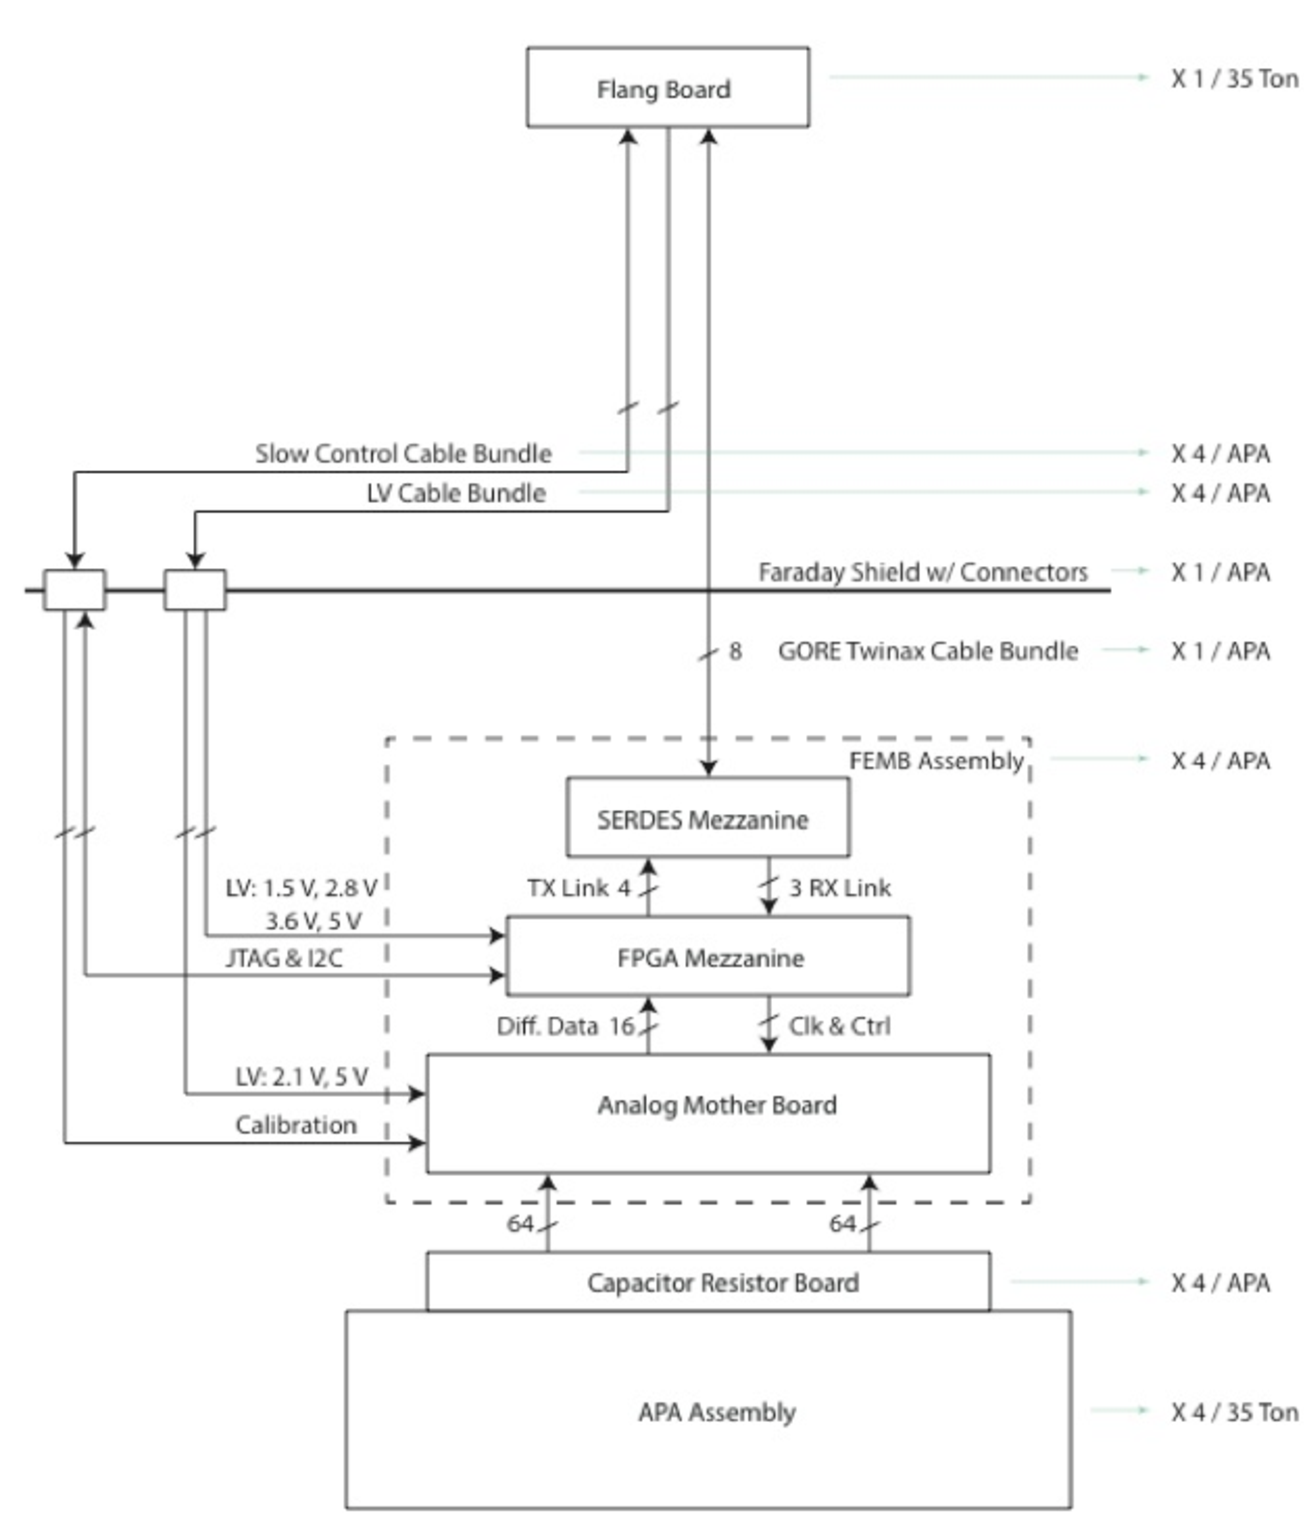
\includegraphics[width=.75\textwidth]{figures/fe-electronics-block-diagram.pdf}
\end{center}
\end{minipage}
\caption{Layout of the TPC cold from end (FE) electronics..}
\label{fig:coldelec}
\end{figure}


Besides the high-speed signal cable, which is a twin-axial cable bundle manufactured by GORE,
there are cable bundles for low-voltage power, wire-bias voltages, and various slow controls and monitoring.
The  cable bundles will be connected through a feedthrough on the roof of the cryostat. 


\begin{figure}[htb]
\centering
\begin{minipage}[b]{1.0\textwidth}
\begin{center}
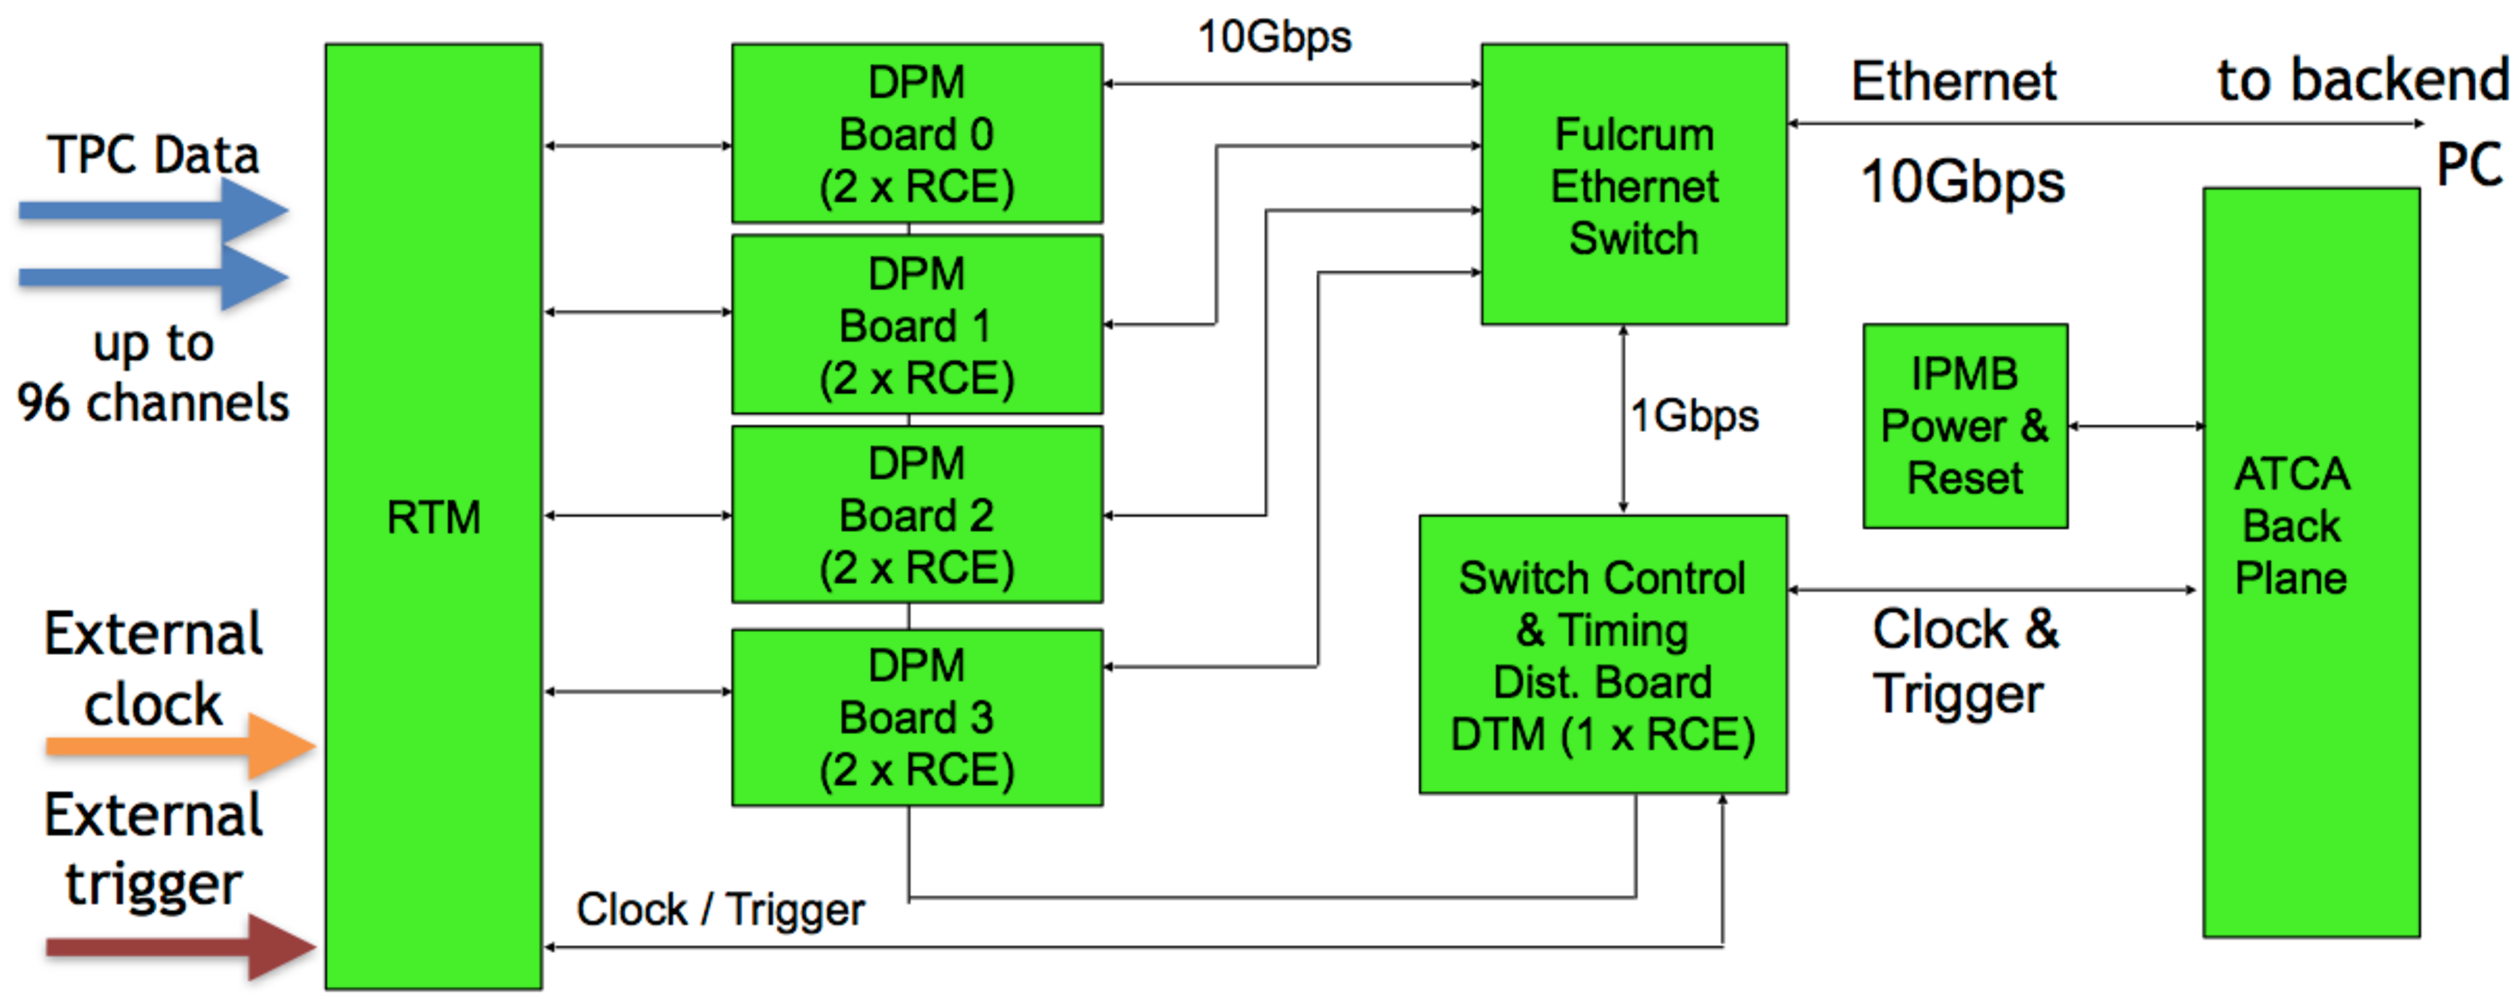
\includegraphics[width=1.0\textwidth]{figures/rce-block.pdf}
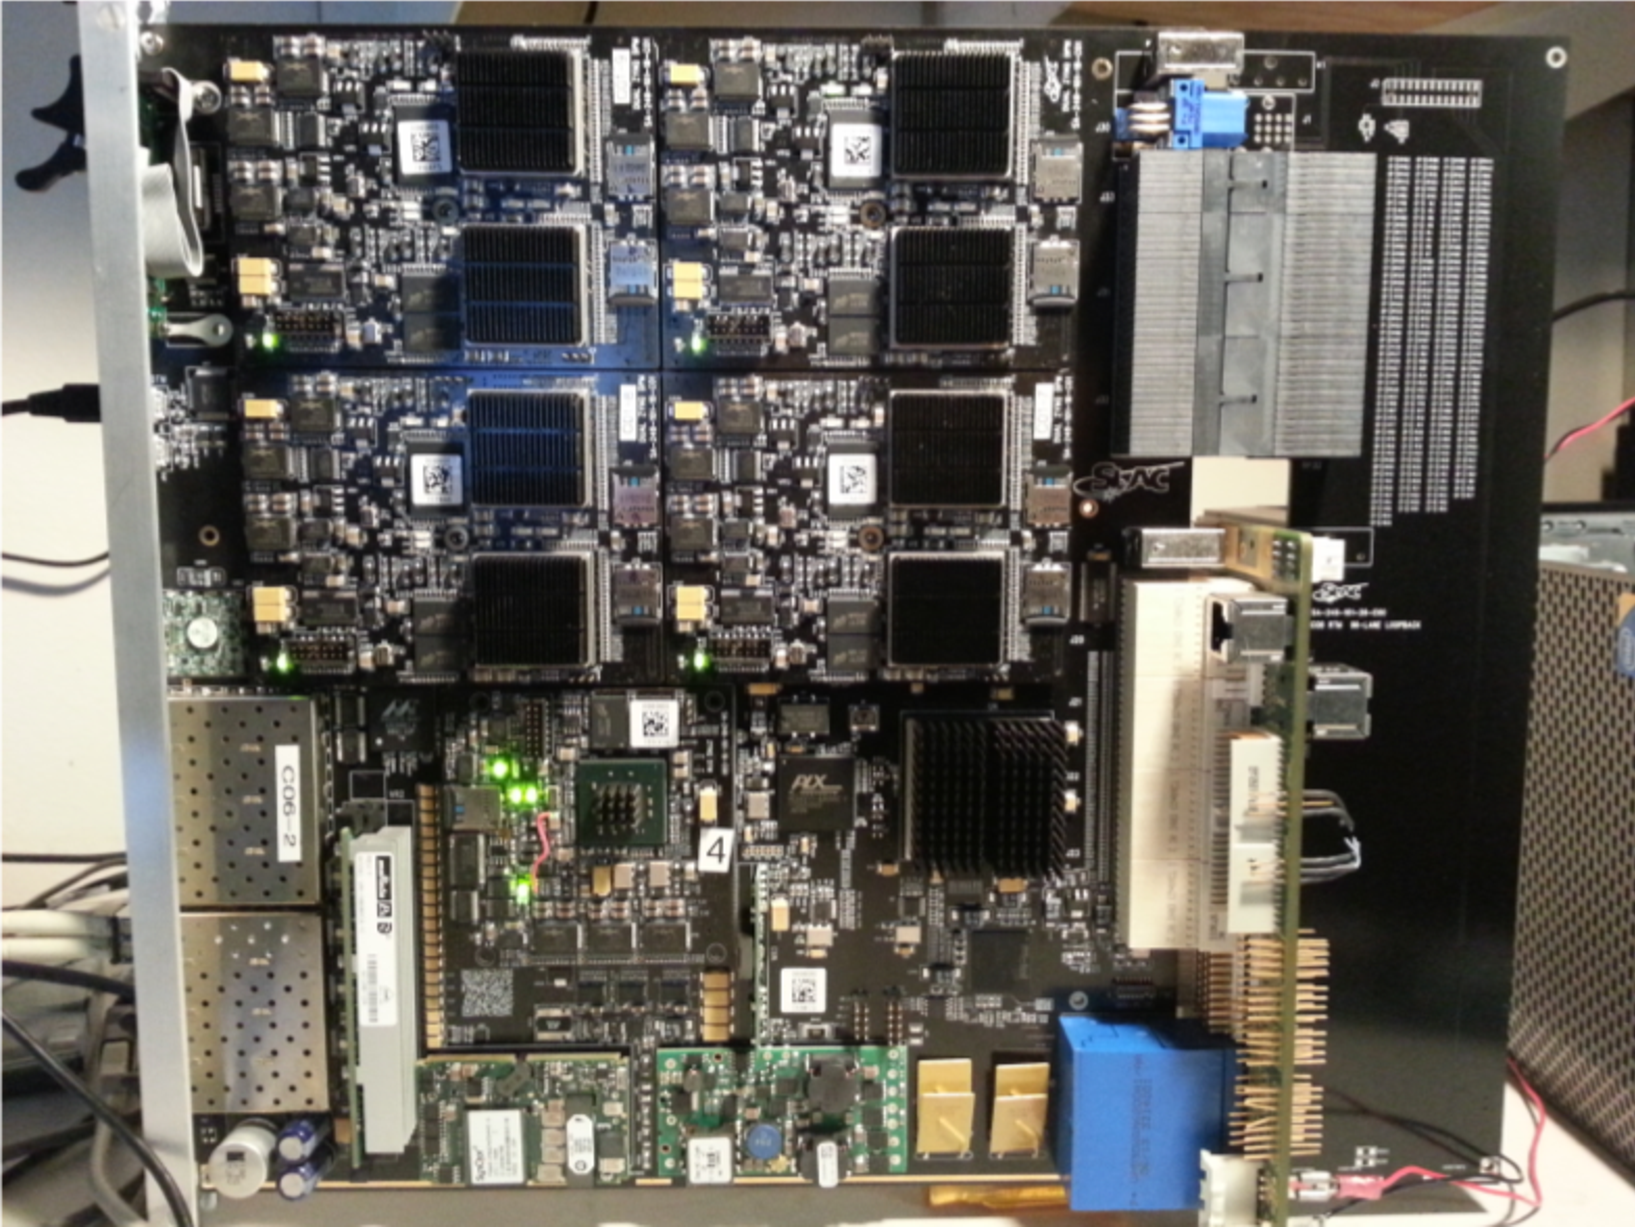
\includegraphics[width=.5\textwidth]{figures/COB-gen3.pdf}
\end{center}
\end{minipage}
\caption{Top: Schematic for the TPC DAQ system. Bottom: The COB (left of the large connectors) and RTM (right).}
\label{fig:rce}
\end{figure}

The primary interface between the TPC front-end electronics (FE) and the DAQ subsystem consists of an ATCA-based system of
RCEs (Reconfigurable Cluster Elements).
The RCE system receives the serialized raw data for the FE, performs zero-suppression on it,
and packetizes and transmits the resulting sparsified data to a back-end data farm for event building and further processing.
Additionally, the RCE system transmits timing and control signals to the FE as well as forwarding configuration data
to them at start-up.     

The RCE system consists of the following components:
a commercial ATCA shelf (2-, 6-, or 14-slot), a Cluster-On-Board (COB) which is the "front board" in ATCA terms,
and a Rear-Transition-Module (RTM) which is the "rear board".
A schematic of the system is shown in Figure \ref{fig:rce}.
The COB is a custom board, developed by SLAC, which holds the processing power of the system.
The COB (see Figure \ref{fig:rce}) consists of 5 bays for holding daughter boards, an onboard 10-GbE switch,
and both 10- and 1-Gb ethernet connections for communications with the back-end system.
Four of the daughter-board bays are for Data Processing Modules (DPM), each of which can hold up to two RCEs.
The RCE is the core procession unit of the system; it is made up of a modern SoC (currently, the Xilinx Zynq-7045)
with multiple high-speed I/O ports (up to 10-Gbps each) and external DRAM and flash memory controllers.
The other bay on the COB contains the Data Transmission Module (DTM) which is responsible
for distributing timing and trigger information to and between the DPMs.  

While the COB hardware is application agnostic, the RTM is application specific.
The RTM provides the mechanical interface between the front-end (or, in our case, the flange electronics)
and the back-end, as well as other external sources such as the timing or trigger systems.
In this case we will use fiber optic connections between the flange and the TPC DAQ using 8 12-channel (full duplex)
CXP connectors on the RTM. 

With the assumption that each cold FE board multiplexes it's 128 wire channels to 4 outputs at 1-Gbps each,
the non-zero suppressed data for 1 APA can be fed into a single COB (containing 8 RCEs).
Each RCE would receive data from 2 FE boards, perform zero-suppression, and send the result to the back-end.  

